\documentclass[12pt]{article}

\usepackage{sbc-template}

\usepackage{graphicx,url}

\usepackage[brazil]{babel}   
\usepackage[utf8]{inputenc} 

\usepackage{amsfonts} 
   
\sloppy

\newcommand{\er}{$\times$}

\title{Avaliação de desempenho de servidores de jogos cooperativos}
\author{Lucas Junqueira Adami (6792496)\inst{1}, Rafael Regis do Prado (6427132)\inst{1}}

\address{
  Instituto de Ciências Matemáticas e de Computação -- Universidade de São Paulo\\
  São Carlos, SP
}

\begin{document} 

\maketitle

\begin{resumo} % 10 linhas
Aplicações distribuídas estão cada dia mais presentes nos sistemas de computação. Em contextos como jogos
cooperativos, a interação entre jogadores se dá por meio de uma rede de
computadores a qual os interliga com um ou mais servidores centrais. Nesses
casos, há o uso intensivo da rede para manter o sincronismo entre os jogadores.
Caso não seja implementada corretamente ou de forma eficiente, a comunicação
entre servidor e jogadores pode ser negativamente impactada, gerando sobrecarga
nos servidores. Este projeto teve como objetivo investigar modos eficientes de
comunicação para jogos cooperativos. Como resultados, foi possível observar
grande diferenças de desempenho entre as abordagens propostas, as quais
variavam parâmetros como o protocolo, o número de jogadores e o tamanho de
pacotes.
\end{resumo}

\section{Introdução} \label{sec:introducao}

Aplicações distribuídas estão cada dia mais presentes nos sistemas de computação. Diversos domínios de
problemas exigem cada vez mais recursos computacionais e necessitam que tarefas
sejam executadas em ambientes distintos. Aplicações numéricas, por exemplo,
pelo alto grau de computação necessário. Muitas vezes, esse tipo de aplicação é
viável apenas quando se é possível utilizar vários núcleos, estejam eles em um
mesmo computador ou em computadores distintos.

Em contextos em que se deve utilizar mais de um computador para realizar
determinada tarefa, a comunicação necessária para a interação dessas tarefas
ocorre tipicamente por meio de uma rede. De fato, certas aplicações só fazem
sentido considerando-se uma rede para a comunicação. Pode-se citar como exemplo
celulares e redes de telefonia móvel, aplicações de compartilhamento de arquivo
e jogos cooperativos.

Para todos os tipos de aplicações e, em especial, para aplicações que fazem uso
intensivo de rede para interação, a eficiência muitas vezes depende de fatores
como o congestionamento de rede, qualidade do serviço de entrega de pacotes,
taxa de mensagens trocadas entre os computadores envolvidos, entre outros.Tais
fatores muitas vezes inviabilizam a utilização da aplicação. Por exemplo, em
uma aplicação de videoconferência, pequenos atrasos na recepção e envio de
\textit{frames} e a perda pontual de certas informações é tolerável. Atrasos
frequentes e contínuos inviabilizam o funcionamento eficaz da mesma.

Em jogos cooperativos \textit{online} ocorre o mesmo. Esse tipo de aplicação
tolera certos atrasos e perdas de informações. No entanto, atrasos constantes
podem resultar em inconsistências na jogabilidade, ou seja, jogadores podem
estar se baseando em um estado desatualizado do jogo para tomar decisões.

Dessa forma, uma das constantes preocupações no desenvolvimento de aplicações
distribuídas está nos padrões de comunicação entre os pares. Assim,
procura-se por técnicas de transmissão de mensagens que sejam eficientes, por
meio da redução da taxa de informações transferidas e por protocolos eficientes
no contexto dessas aplicações.

Este trabalho tem como objetivo investigar cenários favoráveis para aplicações
distribuídas com enfoque em jogos cooperativos. Nas próximas seções serão
abordados a fundamentação teórica para o encaminhamento desse trabalho
(Seção~\ref{sec:fundamentacao}), os objetivos (Seção~\ref{sec:objetivos}), as
atividades desenvolvidas (Seção~\ref{sec:atividades}) e, por fim, os resultados
e conclusões obtidos (Seção~\ref{sec:resultados} e~\ref{sec:conclusoes}).

\section{Fundamentação Teórica} \label{sec:fundamentacao}

Nessa seção, serão abordadas toda a teoria utilizada para o andamento adequado
deste projeto de disciplina. Inicialmente serão abordados os protocolos de
transporte utilizados (Seção~\ref{sub:protocolos}). Em seguida, são
apresentados os modos de execução possíveis através de \textit{sockets} (Seção
~\ref{sub:modos}). Por fim, define-se o padrão de aplicação distribuídas
utilizado nesse trabalho.

\subsection{Protocolos de transporte} \label{sub:protocolos}

No desenvolvimento de aplicações distribuídas, para a comunicação entre os nós
do sistema, utiliza-se como recurso os \emph{sockets}. No contexto de redes de
computadores, \emph{sockets} são definidos como interfaces que possibilitam o
fluxo de dados (envio e recebimento de pacotes de dados) entre dois nós por
meio de uma rede, utilizando uma \emph{API} (\emph{Application Programming
Interface} - Interface de Programação de Aplicativos) definida \cite{Tanenbaum}.

Na perspectiva de camadas de rede, \textit{sockets} representam a interface
entre a camada de aplicação e a de transporte. Nesse sentido, \textit{sockets}
\emph{TCP} (\emph{Transmission Control Protocol}) e \emph{UDP} (\emph{User
Datagram Protocol}) permitem que softwares na camada de aplicação troquem
informações entre si em nível de processos~\cite{Tanenbaum}. Com isso, é
possível desenvolver protocolos na camada de aplicação com a semântica
apropriada para o domínio da aplicação escolhendo o nível de confiabilidade no
transporte dos dados.

Quando há necessidade de se estabelecer uma conexão entre os nós para a
comunicação, a entrega de todos pacotes e na ordem em que foram enviados, é
comum a utilização de protocolos como o \emph{TCP}. Além de prover esses serviços,
esse protocolo oferece ainda controle de congestionamento e de fluxo de dados,
permitindo um uso mais racional da rede que interliga os nós. O protocolo \emph{TCP} é
utilizado, por exemplo, em aplicações que fazem uso do protocolo de aplicação
\emph{Hypertext Transfer Protocol} (\emph{HTTP}~\cite{HTTP}), como navegadores e serviços \emph{Web}.

Por outro lado, quando não há a necessidade de se ter tais garantias ou quando
tais garantias prejudicam o desempenho da aplicação, é utilizado o protocolo
\emph{UDP}. Tal protocolo não disponibiliza os serviços oferecidos pelo protocolo \emph{TCP}.
O que pode parecer uma desvantagem, pode ser útil em situações em que não
importa ordem de pacotes ou que todos os pacotes cheguem. Além disso, em
determinados contextos, o controle de congestionamento pode prejudicar o
desempenho da aplicação~\cite{Kurose}.

Com o protocolo \emph{UDP}, é possível maior controle sobre como os dados são
transportados pela rede, implementando em camada de aplicação os serviços
adequados de forma próxima do necessário para a aplicação em questão. Um
exemplo de aplicação que usa o protocolo \emph{UDP} são os aplicativos de
vídeo-conferência, em que a perda de um \textit{frame} da imagem não é algo
crítico.

\subsection{Modos de Operação de \textit{sockets}} \label{sub:modos}

Dependendo do contexto em que está sendo aplicado, pode-se utilizar diferentes
modos de operação para um determinado \textit{socket}. De fato, existem duas
formas de se utilizar \emph{sockets}: bloqueante e não bloqueante.

Ao se realizar uma operação bloqueante, o nó envolvido interrompe a execução do
programa até que o dado em questão seja enviado ou recebido. Nesse tipo de
comunicação, é garantido que todo o pacote foi devidamente processado a cada
operação de E/S (entrada e saída).

Em seu modo não bloqueante, não há o interrompimento da execução ao se utilizar
o \emph{socket}. A aplicação apenas verifica se há dados a serem escritos ou
lidos antes de realizar um comando nesse modo. Como consequência, é possível
que a operação não seja executada por completo, ou seja, outra operação
sobrescreva aquela em andamento.

Em todos os casos, os diferentes modos de operação de \emph{sockets} podem ser
utilizados para se aumentar o desempenho de aplicações em geral. Tal recurso
pode reduzir significativamente o tempo necessário para se finalizar uma
operação de envio e recebimento de dados, possibilitando melhor utilização de
recursos computacionais.

\textit{Sockets} não-bloqueantes promovem menor ociosidade do processo em
questão com o risco de haver problemas de envio de mensagem. \textit{Sockets}
bloqueantes, por outro lado, asseguram que a mensagem seja totalmente
processada antes de enviá-la havendo, porém, o custo de se esperar o
processamento da mensagem.

% \subsection{Arquitetura Cliente-Servidor} \label{sub:clienteserv}

\section{Objetivos} \label{sec:objetivos}

O objetivo deste trabalho é avaliar o desempenho dos diferentes modos de
operação e protocolos de comunicação disponíveis para \emph{sockets} em
aplicações distribuídas. A avaliação será realizada no contexto de jogos
cooperativos por utilizarem \emph{sockets} para que haja sincronia entre todos
os clientes (jogadores) por meio de servidores.

\section{Atividades Desenvolvidas} \label{sec:atividades}

Para a realização do experimento, uma série de procedimentos foram realizados.
Inicialmente foi realizado o planejamento do experimento
(Seção~\ref{sub:planejamento}) a ser executado para análise da eficiência de
cada configuração proposta. Em seguida, foi especificado o protocolo de
comunicação entre os clientes e o servidor (Seção~\ref{sub:protocolo}) seguido
do desenvolvimento do jogo em si (Seção~\ref{sub:desenvolvimento}). Com o jogo
criado, houve a realização dos experimentos e a análise dos resultados
(Seção~\ref{sub:realizacao}) para que fosse possível verificar a eficácia de
cada configuração.

\subsection{Planejamento do Experimento} \label{sub:planejamento}

Nesta etapa, foram decididos itens fundamentais para a realização do
experimento. Inicialmente, o tipo de jogo (incluindo a natureza das
comunicações a serem realizadas) foi determinado. O jogo escolhido basea-se no
popular jogo \emph{Bomberman}, no qual jogadores podem ativar bombas de modo a
estrategicamente atingir outros jogadores com a explosão da mesma.

A partir do jogo escolhido, determinou-se as variáveis do experimento e
cenários que deveriam ser analisados, tais variáveis podem ser encontradas
abaixo. Com isso, foram planejados os experimentos listados na Tabela~\ref{tab:experimentos}.

\begin{itemize}
  \item \textbf{Protocolo de transporte:} Protocolos \emph{TCP} e \emph{UDP}.
  \item \textbf{Tipo de comunicação:} \emph{Sockets} bloqueantes e não bloqueantes.
  \item \textbf{Tamanho dos pacotes transmitidos:} Pacotes com tamanhos na faixa de 0 a 50 e 100 a 150.
  \item \textbf{Número de jogadores simultâneos:} Cenários com 50 e 100 jogadores simultâneos.
\end{itemize}

\begin{table}
  \center
  \footnotesize
  \begin{tabular}{|c|c|c|c|c|}
  \hline
    \#  & \textbf{Protocolo de transporte} & \textbf{Tipo de comunicação} & \textbf{Tamanho do pacote} & \textbf{Jogadores} \\ \hline
    1 & TCP & Não-bloqueante & 0 & 50 \\ \hline
    2 & TCP & Não-bloqueante & 0 & 100 \\ \hline
    3 & TCP & Não-bloqueante & 100 & 50 \\ \hline
    4 & TCP & Não-bloqueante & 100 & 100 \\ \hline
    5 & TCP & Bloqueante & 0 & 50 \\ \hline
    6 & TCP & Bloqueante & 0 & 100 \\ \hline
    7 & TCP & Bloqueante & 100 & 50 \\ \hline
    8 & TCP & Bloqueante & 100 & 100 \\ \hline
    9 & UDP & Não-bloqueante & 0 & 50 \\ \hline
    10 & UDP & Não-bloqueante & 0 & 100 \\ \hline
    11 & UDP & Não-bloqueante & 100 & 50 \\ \hline
    12 & UDP & Não-bloqueante & 100 & 100 \\ \hline
    13 & UDP & Bloqueante & 0 & 50 \\ \hline
    14 & UDP & Bloqueante & 0 & 100 \\ \hline
    15 & UDP & Bloqueante & 100 & 50 \\ \hline
    16 & UDP & Bloqueante & 100 & 100 \\ \hline
  \end{tabular} 
\caption{Experimentos planejados}
\label{tab:experimentos}
\end{table} 

Em cada experimentos foram observados e medidos os efeitos das configurações no
desempenho do servidor e na comunicação entre o mesmo e os clientes. Desse
modo, o foco do projeto foi em medir a atividade de \emph{CPU}, a quantidade total de
pacotes trocados, o atraso na troca de mensagens e a quantidade de pacotes
perdidos no processo. No contexto de jogos com múltiplos jogadores simultâneos,
a jogabilidade e eficiência do jogo são influenciadas principalmente pelo
atrasos na troca de mensagens e por pacotes perdidos.

Tais experimentos permitirão avaliar o quanto protocolos, quantidade de
jogadores e tamanho de pacotes influenciam nesses fatores. Cada experimento
foi planejado para ser executado 10 vezes, extraindo-se a média das informações
obtidas, totalizando 160 execuções de experimentos.

\subsubsection{Configuração de máquinas utilizada}

Para a execução dos experimentos, optou-se pela utilização do \textit{cluster}
disponível no Laboratório de Sistemas Distribuídos e Programação Concorrente
(LaSDPC). Desse modo, foi utilizada uma máquina virtual para a execução do
servidor e 10 nós físicos para os clientes, cada nó físico executando 10 clientes simultâneos. O uso da máquina virtual ocorreu
devido a necessidade de se instalar programas adicionais para medição dos dados
enviados e recebidos pelo servidor.  As configurações dos nós físicos e máquina
virtual utilizados podem ser visualizadas abaixo.

\textbf{Nós Físicos}

\begin{itemize}
  \item Processador: Core2 Quad Q6600 8MB de Cache 2.40 Ghz
  \item Memória: 8GB DDR3 1333Mhz
  \item HD: Samsung 160GB Samsung 7200 RPM Sata II
  \item Rede: Gigabit Ethernet 
\end{itemize}

\textbf{Nó Virtual}

\begin{itemize}
  \item Processador: 2 CPUs (2.40Ghz cada)
  \item Memória: 4GB de RAM DDR3 1333 Mhz
  \item HD: Virtual de 15GB
  \item Rede: Gigabit Ethernet
\end{itemize}

\subsection{Especificação do Protocolo} \label{sub:protocolo}

Para possibilitar a simulação de um ambiente de jogos cooperativos com
múltiplos jogadores, foi necessário planejar e especificar um possível
protocolo de aplicação para a interação entre os clientes e o servidor.  Dessa
forma, foi criado um conjunto de 14 ações (Tabela~\ref{tab:protocolo}) que
envolvem o envio de mensagem do cliente para o servidor e do servidor para o
cliente.

\begin{table}
  \center
  \footnotesize
  \begin{tabular}{|c|c|c|c|}
  \hline
    \textbf{ID} & \textbf{Nome} & \textbf{Remetente} & \textbf{Campos (seguido do número de bytes)} \\ \hline
    0 & login & Cliente & Nome Jogador(20)  \\ \hline
    1 & add player & Servidor & Identificador(2), Coordenadas X e Y(4), Nome Jogador(20)\\ \hline
    2 & remove player & Servidor & Identificador(2) \\ \hline
    3 & move me & Cliente & Direção(1) (Ex: Norte=0, Leste=2) \\ \hline
    4 & move player & Servidor & Identificador(2), Coordenadas X e Y(4) \\ \hline
    5 & plant bomb & Cliente & \\ \hline
    6 & add bomb & Servidor &  Identificador(2), Coordenadas X e Y(4)  \\ \hline
    7 & explode bomb & Servidor & Identificador (2) \\ \hline
    8 & fall player & Servidor & Identificador (2) \\ \hline
    9 & acknowledge & Cliente & \\ \hline
   10 & ping & Cliente & \\ \hline
   11 & pong & Servidor & \\ \hline
   12 & info & Cliente & Média(16), Desvio Padrão(16), Pacotes Perdidos(4)  \\ \hline
   13 & shutdown & Servidor &\\ \hline
  \end{tabular} 
\caption{Protocolo do jogo criado}
\label{tab:protocolo}
\end{table} 

Para início de interação, cada cliente deve se apresentar para o servidor
através da ação \emph{login} especificando, inclusive, o nome que pretende
utilizar. Como resposta a uma requisição de login, o servidor envia um pacote
\emph{add player} que contém, entre outros dados, o identificador do cliente
corrente permitindo que este possa distinguir-se dos demais jogadores.

Para cada jogador que realiza uma ação de \emph{login}, um pacote de \emph{add player} é enviado para
os demais clientes para que fiquem cientes da presença de um novo jogador. Além
do identificador, são enviados também o nome do jogador e suas coordenadas X e
Y para que cada cliente possa representá-los graficamente e considerá-los ao
realizar suas ações. Da mesma forma, quando um cliente se desconecta, o
servidor envia um pacote \emph{remove player} para que o jogador seja removido localmente.

Quando um jogador desejar se movimentar, deve ser realizada uma ação de \emph{move
me} com a direção desejada. Como resposta, o servidor envia para todos os
clientes um pacote \textit{move player} indicando a nova posição do jogador em
questão ou ainda um pacote \textit{fall player}, caso o jogador saia da arena
(perdendo o jogo).

O mesmo ocorre com as bombas posicionadas na arena do jogo. Ao decidir armar
uma bomba, o cliente envia um pacote \textit{plant bomb} para o servidor, que
atualiza os demais jogadores por meio do envio de pacotes \emph{add bomb} e \emph{explode
bomb} quando a mesma explodir. Por fim, caso o servidor deva ser desligado, o
mesmo avisa com um pacote \textit{shutdown}.

Como pode-se notar, todo o controle sobre o jogo como a física da movimentação
e as regras do jogo permanecem no servidor, restando aos clientes atualizarem
suas próprias informações com base nas informações passadas pelo servidor. Este
cenário é comumente adotado uma vez que reduz a complexidade, permite maior
sincronia entre os jogadores e evita que jogadores mal-intencionados burlem
regras do jogo. Em contrapartida, há uma grande sobrecarga no servidor, que
deve lidar potencialmente com centenas de jogadores simultâneos sem que haja
grandes atrasos na comunicação e faltas de sincronismo entre jogadores.

As ações de 9 a 11 (Tabela~\ref{tab:protocolo}) são ações de controle. A ação
\textit{acknowledge} foi incluída para uniformizar a utilização dos protocolos
de transporte \emph{TCP} e \emph{UDP}. Uma vez que o protocolo \emph{UDP} não estabelece uma
conexão entre os pares, é essencial para o servidor que o cliente avise
periodicamente que ainda está ativo. Com isso, caso não esteja, o servidor pode
descartá-lo de sua tabela de clientes conectados.

As ações de controle \textit{ping}, \textit{pong} e \textit{info} foram
incluídas com a finalidade de se extrair informações úteis a respeito de
pacotes perdidos e atrasos no envio de pacotes para fins estatísticos, algo
especialmente útil para o projeto de redes em questão.

Periodicamente, o cliente envia um pacote \textit{ping} para o servidor, o qual
imediatamente responde com um pacote \textit{pong} permitindo que o cliente
faça medidas do atraso da comunicação. No final, ao receber um pacote
\textit{shutdown} do servidor, o cliente opcionalmente pode enviar a média e
variância dos atrasos e a quantidade de pacotes não recebidos (útil quando
se utiliza protocolo \emph{UDP} para transporte).

Para tratar a questão da perda de pacotes, utilizou-se um campo UID que rotula
unicamente cada pacote com um número crescente. Com isso é possível monitorar
pacotes que chegam no cliente. Caso dois pacotes recebidos tenham a diferença
de UIDs superior a 1, houve uma perda de pacote. Note que pacotes podem chegar desordenados. Portanto, esse valor obtido pode ser maior que o total real de pacotes perdidos.

\subsection{Desenvolvimento de Jogo Cooperativo} \label{sub:desenvolvimento}

O desenvolvimento do jogo foi separado em duas partes: implementação do
servidor e implementação do cliente. Como linguagens de programação, foram
utilizadas \emph{C++} \cite{CPP} para a implementação do servidor e \emph{Java} \cite{Java} para a implementação dos
clientes.  O projeto inteiro foi desenvolvido utilizando-se a ferramenta de
versionamento \emph{Git} \cite{Git}. O código do projeto, modo de instalação e experimentos podem
ser encontrados em https://github.com/rafaelregis/bomberboys .

O teste das funcionalidades pôde ser feito por meio do desenvolvimento do modo
gráfico em conjunto com o servidor. Utilizando-se tal modo foi possível
verificar a interação entre os clientes (jogadores) por meio do servidor assim
como a influência das regras do jogo sobre os mesmos. Um exemplo de partida
utilizando-se 10 jogadores pode ser visualizado na Figura~\ref{fig:partida}. As
bombas são representadas pelos quadrados menores enquanto os jogadores são
representados pelos quadrados maiores com circulos internos. A arena está
contida no retângulo com borda verde.

\begin{figure}[ht]
  \centering
  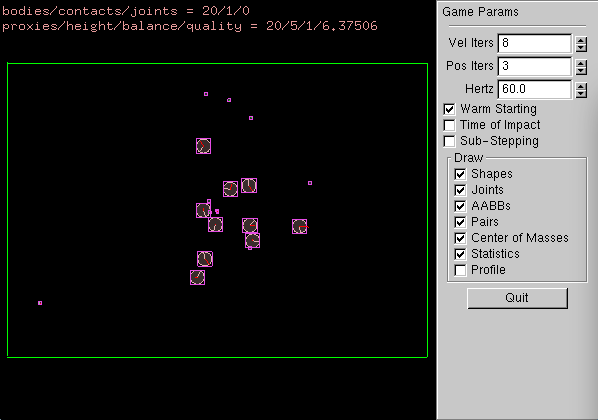
\includegraphics[width=.8\textwidth]{img/partida.png}
  \caption{Exemplo de partida do jogo desenvolvido}
  \label{fig:partida}
\end{figure}

\subsubsection{Desenvolvimento do Servidor de Jogos}

O servidor desenvolvido possui quatro modos de operação. São eles: \emph{TCP}
bloqueante, \emph{TCP} não bloqueante, \emph{UDP} bloqueante e \emph{UDP} não
bloqueante. Na Figura~\ref{fig:server}, a maneira como cada modo é implementado
é mostrada. Para o \emph{TCP} não bloqueante, há uma única \emph{thread}
responsável pelo gerenciamento de todos os \emph{sockets}. Nesse modo, há um
\emph{socket} principal, \emph{SS}, que recebe novas conexões. A cada conexão
estabelecida, um novo \emph{socket} \emph{Si} é criado para manter a conexão
com o cliente \emph{i}.

No modo \emph{TCP} bloqueante, há uma \emph{thread} responsável pelo
recebimento de novas conexões por meio do \emph{socket} \emph{SS} e duas
\emph{threads} de leitura e escrita para cada cliente. Ambos os modos que
utilizam \emph{TCP} identificam seus clientes por meio do \emph{file
descriptor} (\emph{FD}) do \emph{socket} aberto na conexão. 

Para o \emph{UDP} não bloqueante, o único \emph{socket} utilizado é o \emph{SS}. Há uma única \emph{thread} responsável por processar pacotes recebidos e a serem enviados. Nos modos \emph{UDP}, não há conexão. Portanto, não existe um \emph{FD} para
cada cliente. Desta forma, os clientes são identificados pelo par \emph{IP} e
porta no servidor. 

No modo \emph{UDP} bloqueante, há uma \emph{thread}
responsável pela leitura de pacotes de todos os clientes por meio do
\emph{socket} \emph{SS} e uma \emph{thread} de escrita para cada cliente e que
compartilha o \emph{socket} \emph{SS}. 

\begin{figure}[ht]
  \centering
  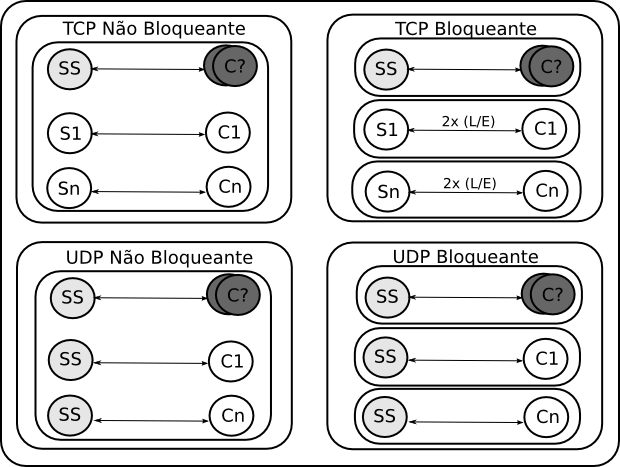
\includegraphics[width=.8\textwidth]{img/server.png}
  \caption{Modos de operação do servidor}
  \label{fig:server}
\end{figure}

\subsubsection{Desenvolvimento dos Clientes}

Para tornar a inicialização de processos clientes prática para fins de
experimentação, foi implementado um programa que permite a inicialização
simultânea de um número variável de clientes, de acordo com o experimento sendo
realizado. Internamente, é inicializado um conjunto de \textit{threads} para
cada cliente e cada um desses se comunica com o servidor por seu próprio
\textit{socket}.

Além do número de clientes a serem inicializados, foi possível configurar o
protocolo de transporte e o tamanho das mensagens a serem enviadas. A questão
do modo em que os \textit{sockets} operam (bloqueante e não-bloqueante) não foi
variável nos clientes. De fato, o modo não-bloqueante faz sentido apenas no
servidor. Clientes devem esperar para receber informações de um (único)
servidor de modo que, caso fosse implementada a abordagem não bloqueante, seria
necessária uma espera ocupada o que, no fim, simula o modo bloqueante.

Para que fosse possível a simulação de uma partida do jogo utilizando o
servidor e os clientes, foi criado um \textit{bot} (jogador artificial) o qual
joga de forma aleatória. No contexto do experimento, há até 100
jogadores simultâneos.  A utilização de \textit{bots} com inteligência
artificial ou de jogadores humanos dificilmente acarretaria em resultados
diferentes uma vez que o espaço da arena do jogo inviabiliza a utilização de
estratégias elaboradas com essa quantidade de jogadores.

\subsection{Realização de Experimentos e Análise dos Resultados} \label{sub:realizacao} 

A partir do jogo desenvolvido, cada um dos 16 experimentos foi executado 10
vezes no \textit{cluster}, como especificado em~\ref{sub:planejamento}. Foram
criados e distribuídos para os nós do cluster uma série de \textit{scripts}
com os parâmetros de interesse devidamente especificados (número de clientes a
serem iniciados na máquina, protocolo de transporte etc).

Com isso, a partir de um determinado nó do \textit{cluster}, o servidor do jogo
foi criado e, por meio de acessos \emph{SSH} automatizados, os clientes foram criados
em outros nós em seguida, todo o processo conforme o especificado para o
experimento selecionado.

Para cada execução de experimento, foram armazenados dados como a quantidade
total de \emph{bytes} trocados entre o servidor e seus clientes, a carga da \emph{CPU}
durante o experimento, a média e variância do atraso na comunicação e a
quantidade de pacotes perdidos em disco para análise posterior. Desse total de
dados, foram extraídas as informações de interesse por meio de
\textit{scripts}.

Uma dificuldade encontrada no trabalho foi o desenvolvimento do cliente utilizando a linguagem \emph{Ruby}. Nos experimentos, 10 clientes eram executados ao mesmo tempo em cada máquina. Por fatores de desempenho dessa linguagem, a máquina ficava lenta e os resultados dos experimentos eram inconsistentes. Por causa desse problema, os clientes foram desenvolvidos em \emph{Java}.

Outra resistência encontrada foi a dificuldade da utilização do \emph{cluster}. Inicialmente, os arquivos estavam na pasta do usuário (\emph{home}) e por questões de configuração do sistema de arquivos os experimentos ficavam lentos, resultando em valores errôneos. Ao passar os arquivos para a pasta \emph{opt} das máquinas, as execuções fluíram de maneira normal. 

Os resultados obtidos podem ser observados em~\ref{sub:dados} e as conclusões a
respeito dos mesmos podem ser analisadas em~\ref{sub:discussao}.

\section{Resultados} \label{sec:resultados}

Nessa Seção, os resultados obtidos a partir dos experimentos realizados são mostrados. Ainda, uma discussão desses valores é feita. Uma análise das falhas nos experimentos também é comentada.

\subsection{Dados Obtidos} \label{sub:dados}

Na Tabela~\ref{tab:resultados}, os resultados dos experimentos estão ilustrados. A primeira coluna representa os identificadores dos experimentos que podem ser consultados na Tabela~\ref{tab:experimentos}. A segunda e terceira colunas representam as médias do atraso e variância percebidos nos clientes, respectivamente. A quarta coluna \emph{CPU}, mostra a utilização da \emph{CPU} no modo usuário, no modo \emph{kernel} e a ociosidade da máquina do servidor. A quinta coluna, \emph{bytes}, possui dois valores que equivalem ao número de \emph{bytes} enviados e recebidos pelo servidor. A última coluna indica o número de pacotes perdidos. Os dados de \emph{CPU} e \emph{bytes} recebidos e enviados foram obtidos por meio dos programas presentes no \emph{Linux} chamados \emph{vmstat} \cite{Vmstat} e \emph{nstat} \cite{nstat} respectivamente. No segundo programa, os valores foram extraídos a partir dos campos \emph{IpExtInOctets} e \emph{IpExtOutOctets}.

\begin{table}
  \center
  \footnotesize
  \begin{tabular}{|c|c|c|c|c|c|}
  \hline
  \# & \textbf{Atraso ($ms$)} & \textbf{Variância ($ms$)} & \textbf{CPU (\%)} & \textbf{Bytes (enviado/recebido)} & \textbf{Pacotes Perdidos} \\ \hline
    1 & 50.04 & 1.74 & 16.1/9.6/73.6 & 21688636.2/438917162.9 & 0 \\ \hline
    2 & 302.68 & 192.15 & 27.8/7.2/63.83 & 21998667.43/380864913.9 & 0 \\ \hline
    3 & \er & \er & \er & \er & \er \\ \hline
    4 & \er & \er & \er & \er & \er \\ \hline
    5 & 50.16 & 3.14 & 31/25.6/43 & 20717318.5/310870796.8 & 0 \\ \hline
    6 & 53.89 & 12.08 & 33.15/31.5/34.75 & 35965675.65/375906838.45 & 0 \\ \hline
    7 & 50.02 & 0.53 & 23.4/44.2/32.2 & 66501124.9/2064695664.9 & 0 \\ \hline
    8 & 54.15 & 9.52 & 23.55/47.35/28.9 & 77556161.35/2327154624.80 & 0 \\ \hline
  \end{tabular} 
\caption{Resultados dos experimentos}
\label{tab:resultados}
\end{table} 

Na Figura~\ref{fig:delay-graph}, os tempos de atraso e suas variâncias para os experimentos executados estão apresentados. O eixo $x$ representa o número do experimento e o eixo $y$ o tempo em milisegundos.

\begin{figure}[ht]
  \centering
  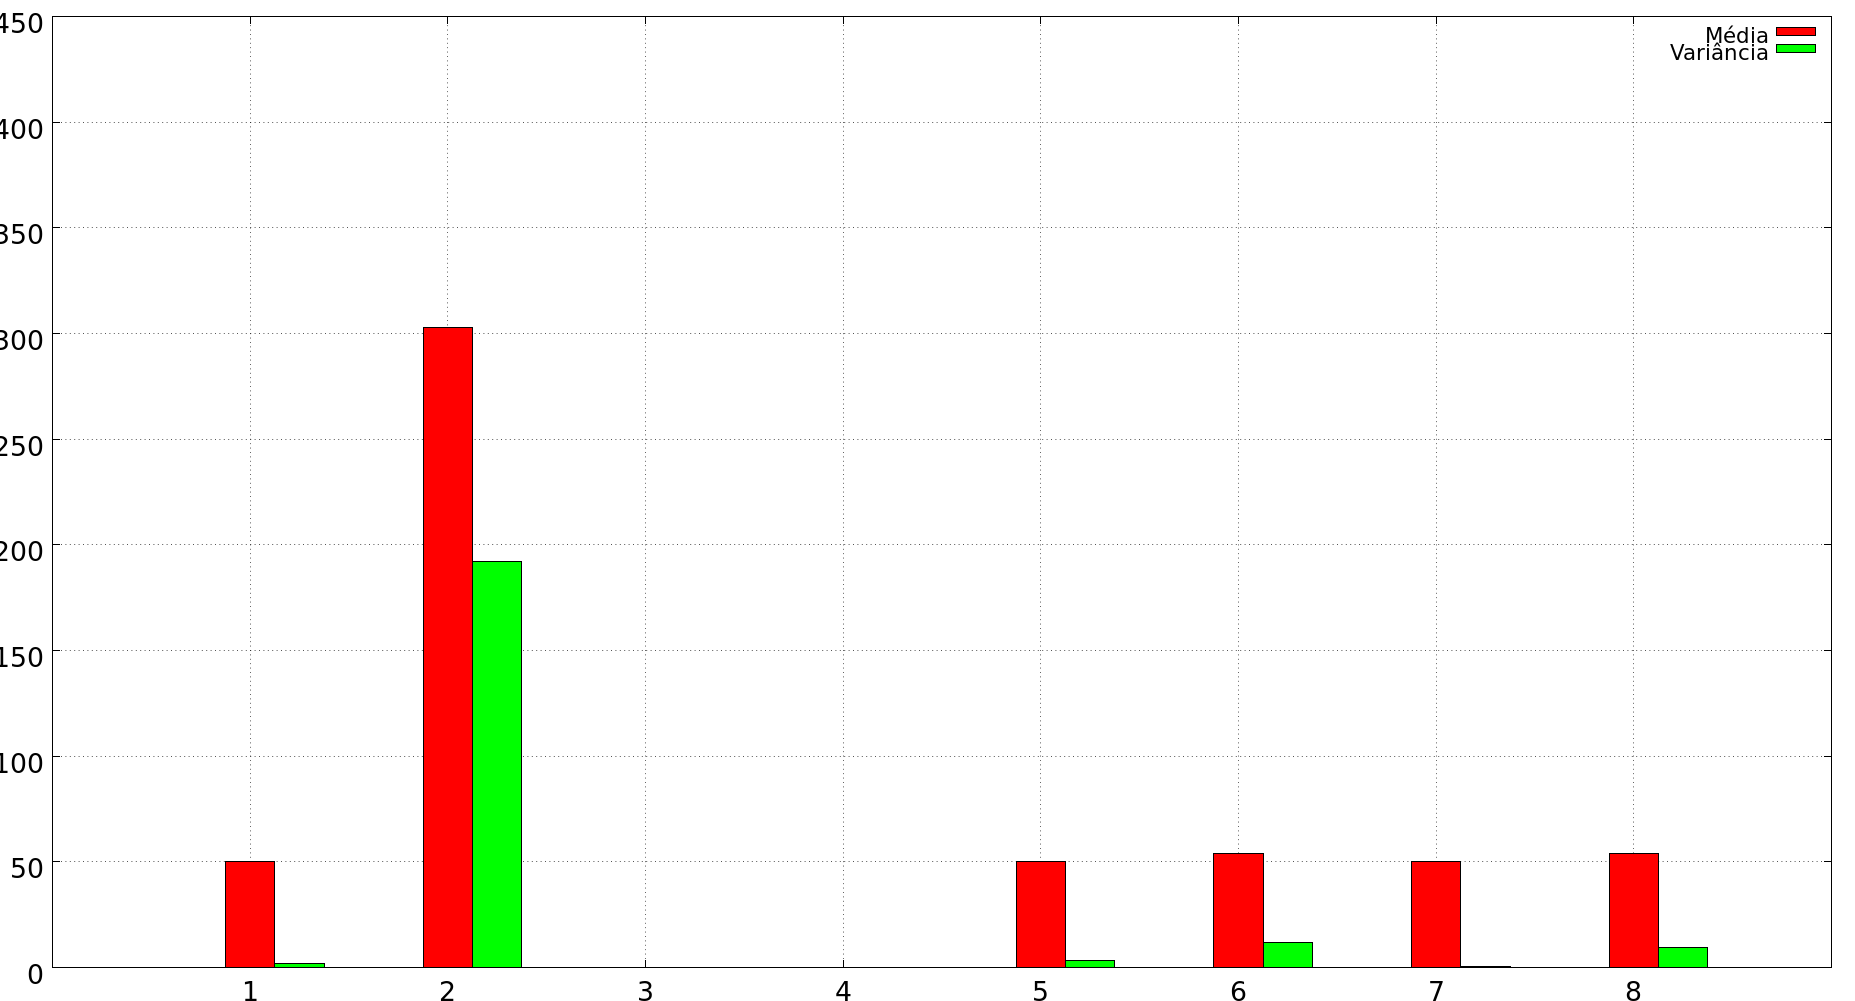
\includegraphics[width=1\textwidth]{img/delay-graph.png}
  \caption{Tempos de atraso}
  \label{fig:delay-graph}
\end{figure}

Na Figura~\ref{fig:cpu-graph}, as cargas de \emph{CPU} na máquina do servidor dos experimentos executados estão à mostra. O eixo $x$ mostra o experimento correspondente enquanto o eixo $y$ indica a porcentagem dos valores de utilização nos modos usuário, \emph{kernel} e ocioso.

\begin{figure}[ht]
  \centering
  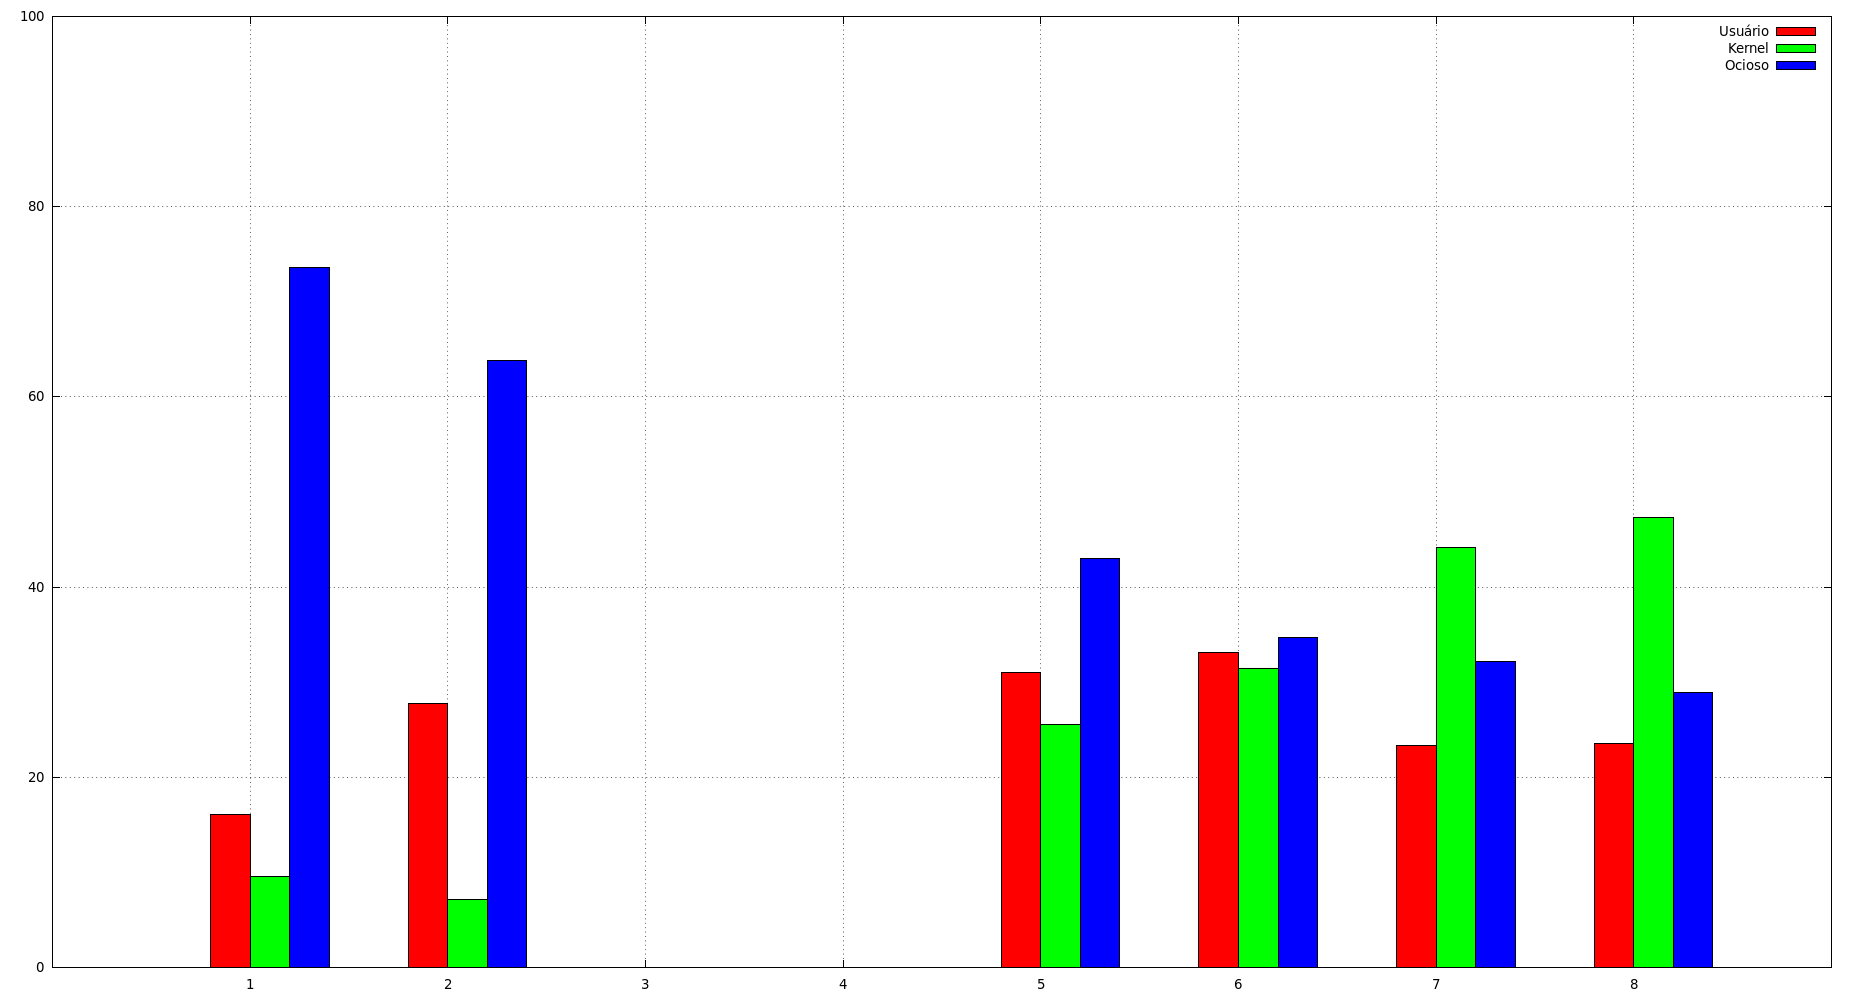
\includegraphics[width=1\textwidth]{img/cpu-graph.png}
  \caption{Cargas de \emph{CPU}}
  \label{fig:cpu-graph}
\end{figure}

A quantidade de \emph{bytes} enviados e recebidos pelo servidor durante os experimentos está ilustrada na Figura~\ref{fig:net-graph}. No eixo $x$, o experimento está indicado. Os valores dessas métricas estão representados no eixo $y$.

\begin{figure}[ht!]
  \centering
  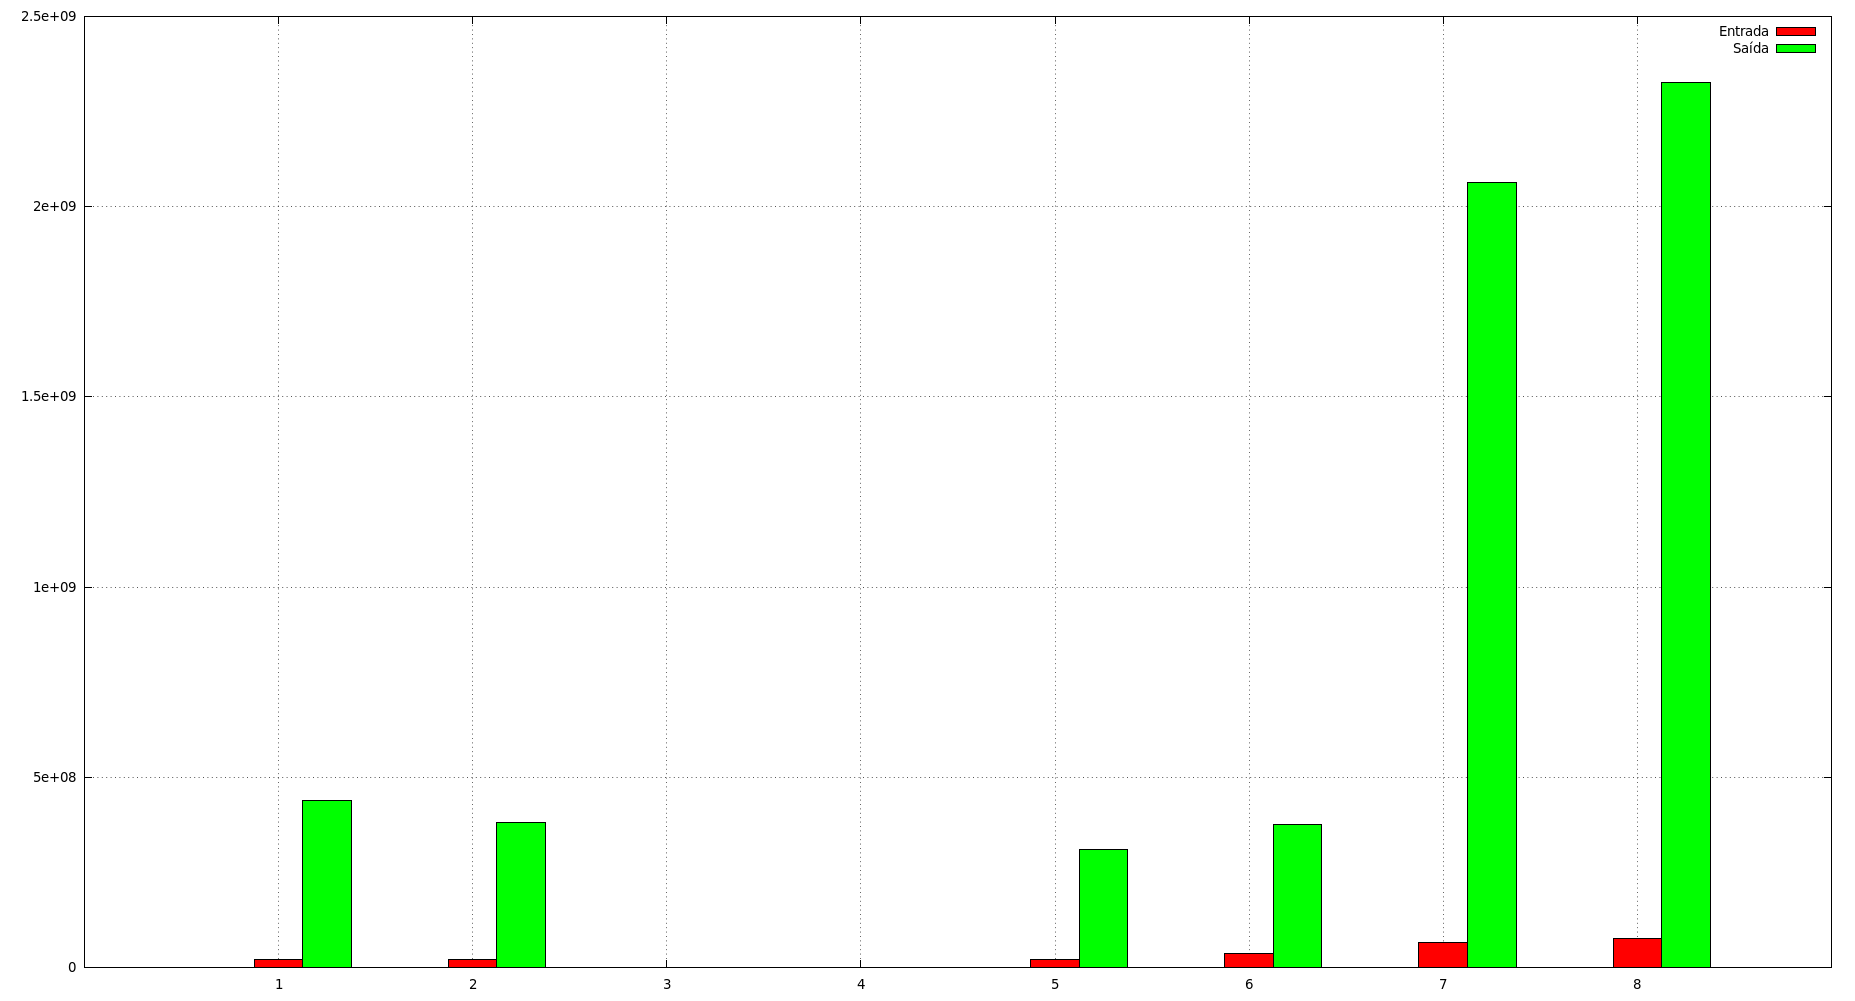
\includegraphics[width=1\textwidth]{img/net-graph.png}
  \caption{\emph{Bytes} enviados e recebidos}
  \label{fig:net-graph}
\end{figure}

Na Figura~\ref{fig:tcp-graph}, os tempos de atraso e suas variâncias para o jogo sendo executado no modo \emph{TCP} não bloqueante com pacotes de tamanho mínimo 100 estão apresentados. O eixo $x$ mostra o número de clientes conectados e o eixo $y$ o tempo em milisegundos. A curva gerada é aproximada por curvas de \emph{Bezier} \cite{Bezier}.

\begin{figure}[ht]
  \centering
  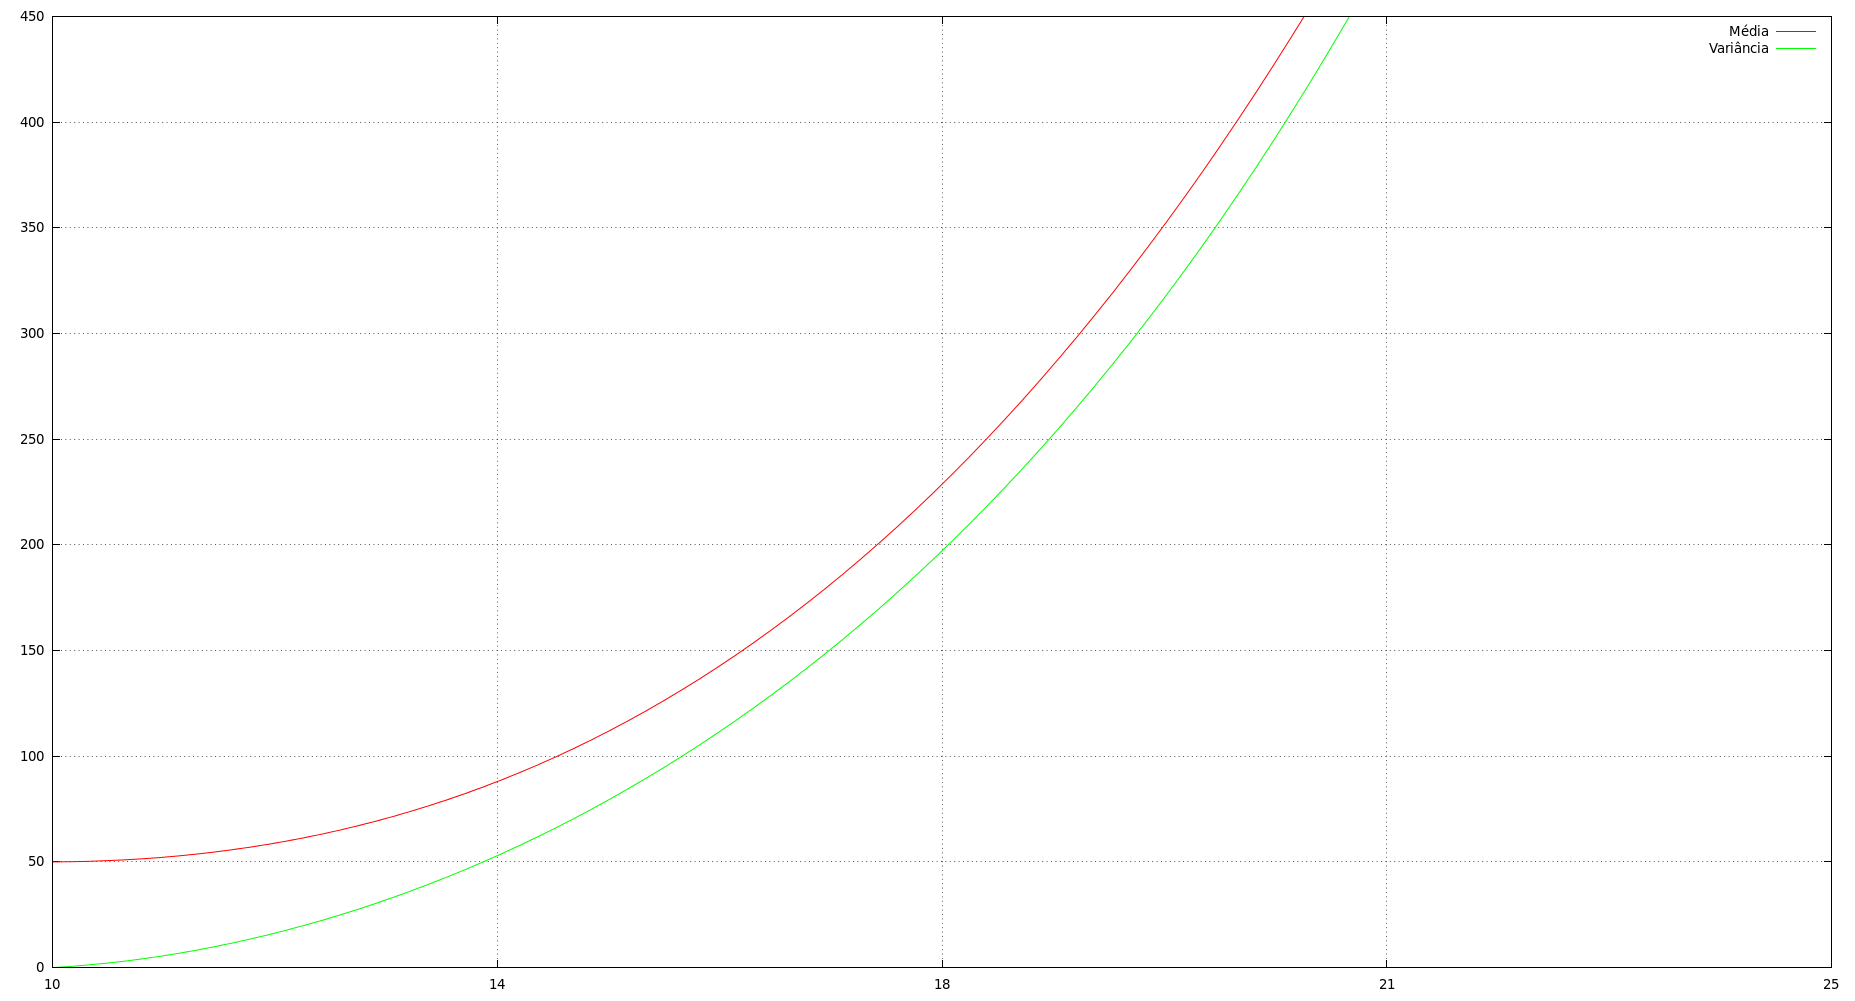
\includegraphics[width=1\textwidth]{img/tcp-graph.png}
  \caption{Tempos para o modo \emph{TCP} não bloqueante}
  \label{fig:tcp-graph}
\end{figure}

\subsection{Discussão dos Resultados} \label{sub:discussao}

No decorrer da execução dos experimentos referentes ao protocolo \emph{UDP},
percebeu-se uma alta perda pacotes mesmo para casos simples com até 10 clientes
que, em média, levava a uma perda de até 70000 pacotes. Dessa forma, para os
parâmetros previamente estabelecidos (50 e 100 clientes), o experimento com
esse protocolo foi inviável, já que perdia-se, inclusive, pacotes de controle
do protocolo do jogo. 

Essa perda de pacotes pode ser explicada pelo fato de o protocolo \emph{UDP},
além de não garantir na entrega de pacotes, não oferecer serviços de controle
de congestionamento e de fluxo. Com isso, houve uma inundação de pacotes nos
clientes e principalmente nos servidores, degradando a comunicação entre os
pares.

O fenômeno da alta perda de pacotes observadas nos experimentos não foi
inicialmente prevista. Por isso, tinha-se como objetivo apenas a troca o
protocolo \emph{TCP} pelo \emph{UDP} tolerando-se eventuais perdas de pacotes,
o que não degradaria a experiência do jogo nem interferiria drasticamente no
controle dos experimentos.

Apesar de o projeto ter como foco, entre outros, a investigação do protocolo
\emph{UDP} como alternativa viável, estes experimentos seriam viáveis caso
houvesse a implementação do controle de fluxo e de congestionamento em nível de
aplicação, o que foge do escopo proposto inicialmente.

Na Tabela~\ref{tab:resultados}, pode-se observar que o atraso médio dos
experimentos não variou muito com a alteração do número de clientes e o tamanho
mínimo dos pacotes, com exceção de um caso, comentado logo abaixo. A variância
seguiu a mesma tendência, não variando muito com o aumento de clientes e
tamanho de pacotes.

A carga no servidor foi maior para \emph{TCP} bloqueante em todos os
experimentos. Esse resultado já era esperado, pois com o número alto de
\emph{threads} criadas, há uma sobrecarga na troca de contexto entre elas. 

O número de \emph{bytes} enviados e recebidos seguiu a tendência esperada ao
aumentar quando o número de clientes e tamanho mínimo do pacote cresceram.
Novamente, uma exceção a essa regra ocorreu e é comentada a seguir. Ainda, essa
taxa de aumento não foi proporcional ao aumento da carga nos experimentos, o
que somente pode ser justificado estudando-se como funciona a ferramenta
utilizada para a coleta desses valores, o \emph{nstat}.

Como representado na Tabela~\ref{tab:resultados}, não foi possível extrair
resultados dos experimentos 3 e 4. Além disso, o resultado do experimento 2 não
seguiu o esperado nesse tipo de execução (os experimentos 2, 3 e 4 são do tipo
\emph{TCP} não bloqueante). O resultado do experimento 2 não entrou na
análise deste trabalho, pois foi considerado como anômalo. Foi possível
analisar, no entanto, um grande estresse no sistema ao se executar os
experimentos 3 e 4, o que inviabilizou a avaliação dos resultados.

Para se analisar a possível causa desses problemas relatados, foram realizados
experimentos adicionais envolvendo o protocolo \emph{TCP} no modo não
bloqueante com tamanho mínimo de pacotes 100. Esses experimentos estão
ilustrados na Figura~\ref{fig:tcp-graph}. Foi possível observar que há, para
esses casos, uma relativa estabilidade na execução para até uma certa
quantidade de jogadores. A partir de uma determinada quantidade, o servidor não
escala com a quantidade de requisições, entrando, de certa forma, em colapso.

Para todos os casos analisados a fundo, tal fenômeno ocorre na faixa de 20
clientes simultâneos. A utilização máxima da \emph{CPU} é descartada como
causa desse problema, pois o tempo de ociosidade verificado nos experimentos
foi alto (para 21 clientes, esse valor foi de 78\%). Outras análises devem ser
feitas para se justificar a causa a causa desses tempos de atraso.

Com relação aos os tempos médios de atraso, houve pouca variação sendo que
estes ficaram próximos a 50$ms$. Esse valor (50$ms$) é o mínimo possível por ser
o valor de espera interno (antes de processar novos pacotes) na implementação
do cliente. Finalmente, o número de pacotes perdidos para todos
os casos \emph{TCP} foi de 0, algo esperado por se tratar de um protocolo de
camada de transporte que garante a entrega de todos os pacotes na ordem.

\section{Conclusões} \label{sec:conclusoes}

Tendo-se em vista os dados obtidos e as discussões a respeito da influência dos
fatores sobre a qualidade do serviço (tempo de transferência, trafego de dados
etc) discutidos na seção~\ref{sec:resultados}, pode-se recomendar certas
abordagens na comunicação entre pares em um ambiente de jogos cooperativos.

Como pôde ser notado, a utilização do protocolo \emph{UDP} de forma pura não
pode ser aplicado para a comunicação entre cliente e servidor. Apesar desse
tipo de aplicação tolerar perdas eventuais de pacotes, quando se trata de
dezenas ou centenas de clientes interagindo pelo servidor, a perda de dados
será muito elevada, levando o sistema como um todo ao colapso.

No entanto, pode-se recomendar o protocolo \emph{UDP} em casos em que não é
necessário o controle estatístico, em cenários em que há menos que 10 clientes
ou ainda quando se dispõe minimanente de um controle de fluxo e
congestionamento em nível de aplicação.

Para o contexto de jogos cooperativos, com pacotes de controle, o melhor
protocolo a ser utilizado é o \emph{TCP}, porque o \emph{UDP} com certeza
perderá muitos pacotes essenciais. O modo não bloqueante utiliza menos carga da
\emph{CPU} e é mais fácil de programar, por não envolver necessariamente
concorrência, obtendo-se resultados bastante satisfatórios em termos de
desempenho.

Para o caso de estudo foco desse projeto, resultados mostraram que a partir de
um número de clientes, a abordagem não bloqueante passou a gerar atrasos muito
grandes. Considerando esse fato, é mais seguro utilizar a abordagem bloqueante
que, para os experimentos realizados, demonstrou maior estabilidade nesse
sentido.

Não foi possível se extrair informações mais precisas a partir dos experimentos
executados devido a fatores não considerados que, de fato, geraram grande
impacto de performance principalmente nos casos em que o modo de execução era
não bloqueante. Acredita-se que tal abordagem seja mais efetiva de maneira
geral que a abordagem bloqueante uma vez que reduz-se custos na espera
bloqueante para envio e recebimento de pacotes. Constata-se no entanto a
presença de outros fatores não investigados nesse projeto que afetam
diretamente aplicações desse tipo.

Como trabalhos futuros, sugere-se principalmente a investigação de novos
fatores que impactam diretamente na performance de servidores desse tipo.
Outras possibilidades incluem a realização de experimentos utilizando-se a
\emph{Internet}, validando as hipóteses para o cenário em que ocorre a troca de
pacotes em um jogo colaborativo. Por fim, experimentos podem ser realizados
tendo-se como base um protocolo, possivelmente na camada de aplicação, sem
conexão como o \emph{UDP} mas com garantias de controle de fluxo e de
congestionamento, por exemplo, algo que se mostrou necessário nos experimentos
realizados nesse projeto.

\bibliographystyle{sbc}
\bibliography{bibliography}

\end{document}
